\documentclass{beamer}

\title{NWEN304 Interim Presentation}
\subtitle{Turtles all the way down}
\author{Colin \and Greg}
\subject{Computer Science}

\AtBeginSection[]{
  \begin{frame}
  \vfill
  \centering
  \begin{beamercolorbox}[sep=8pt,center,shadow=true,rounded=true]{title}
    \usebeamerfont{title}\insertsectionhead\par%
  \end{beamercolorbox}
  \vfill
  \end{frame}
}

\date{}

\begin{document}
  \begin{frame}
    \titlepage
  \end{frame}

  % Frames for screenshots
  \begin{frame}
    \frametitle{Frontend}
    \begin{figure}[h]
      \centering
      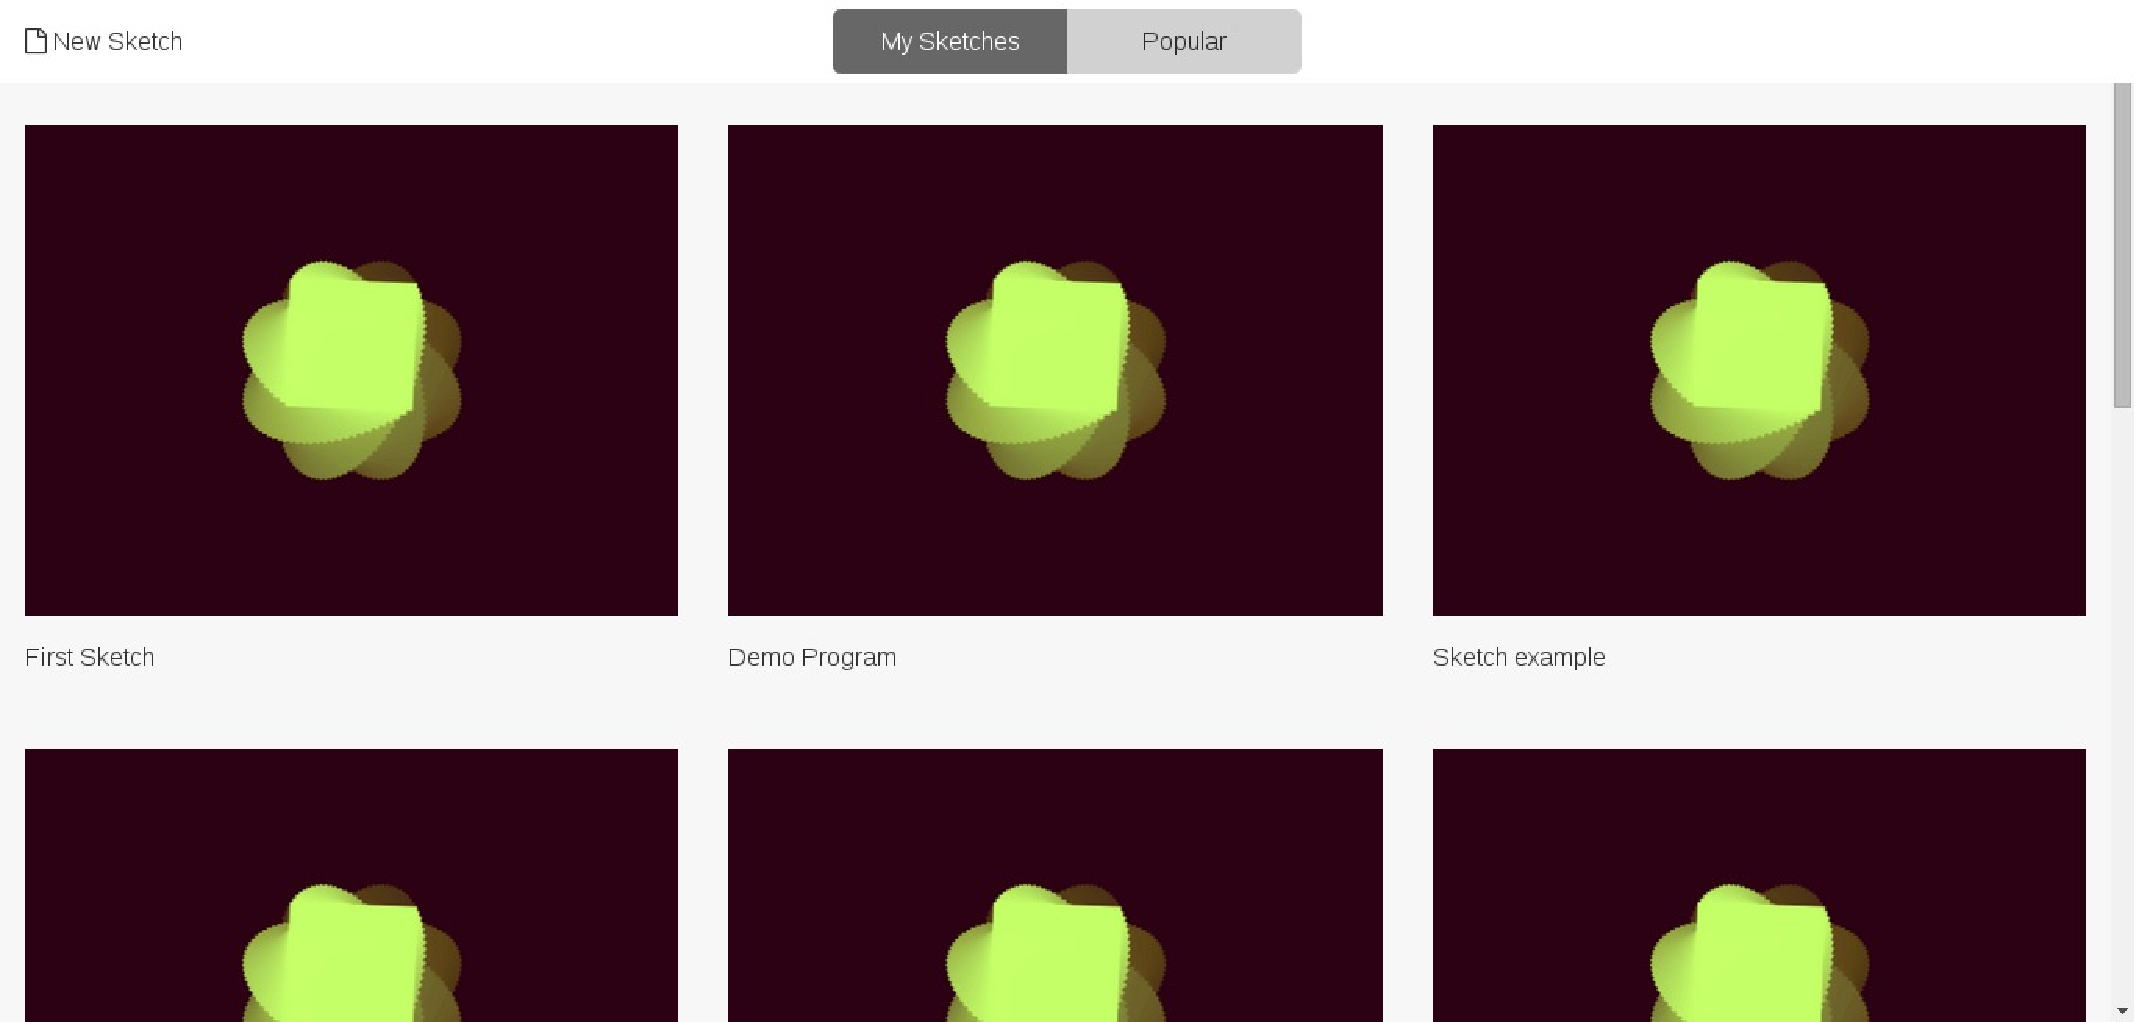
\includegraphics[width=\textwidth,keepaspectratio]{browser.pdf}
      \caption{Sketch Browser}
      \label{fig:axbgrid}
    \end{figure}
  \end{frame}

  \begin{frame}
    \frametitle{Frontend}
    \begin{figure}[h]
      \centering
      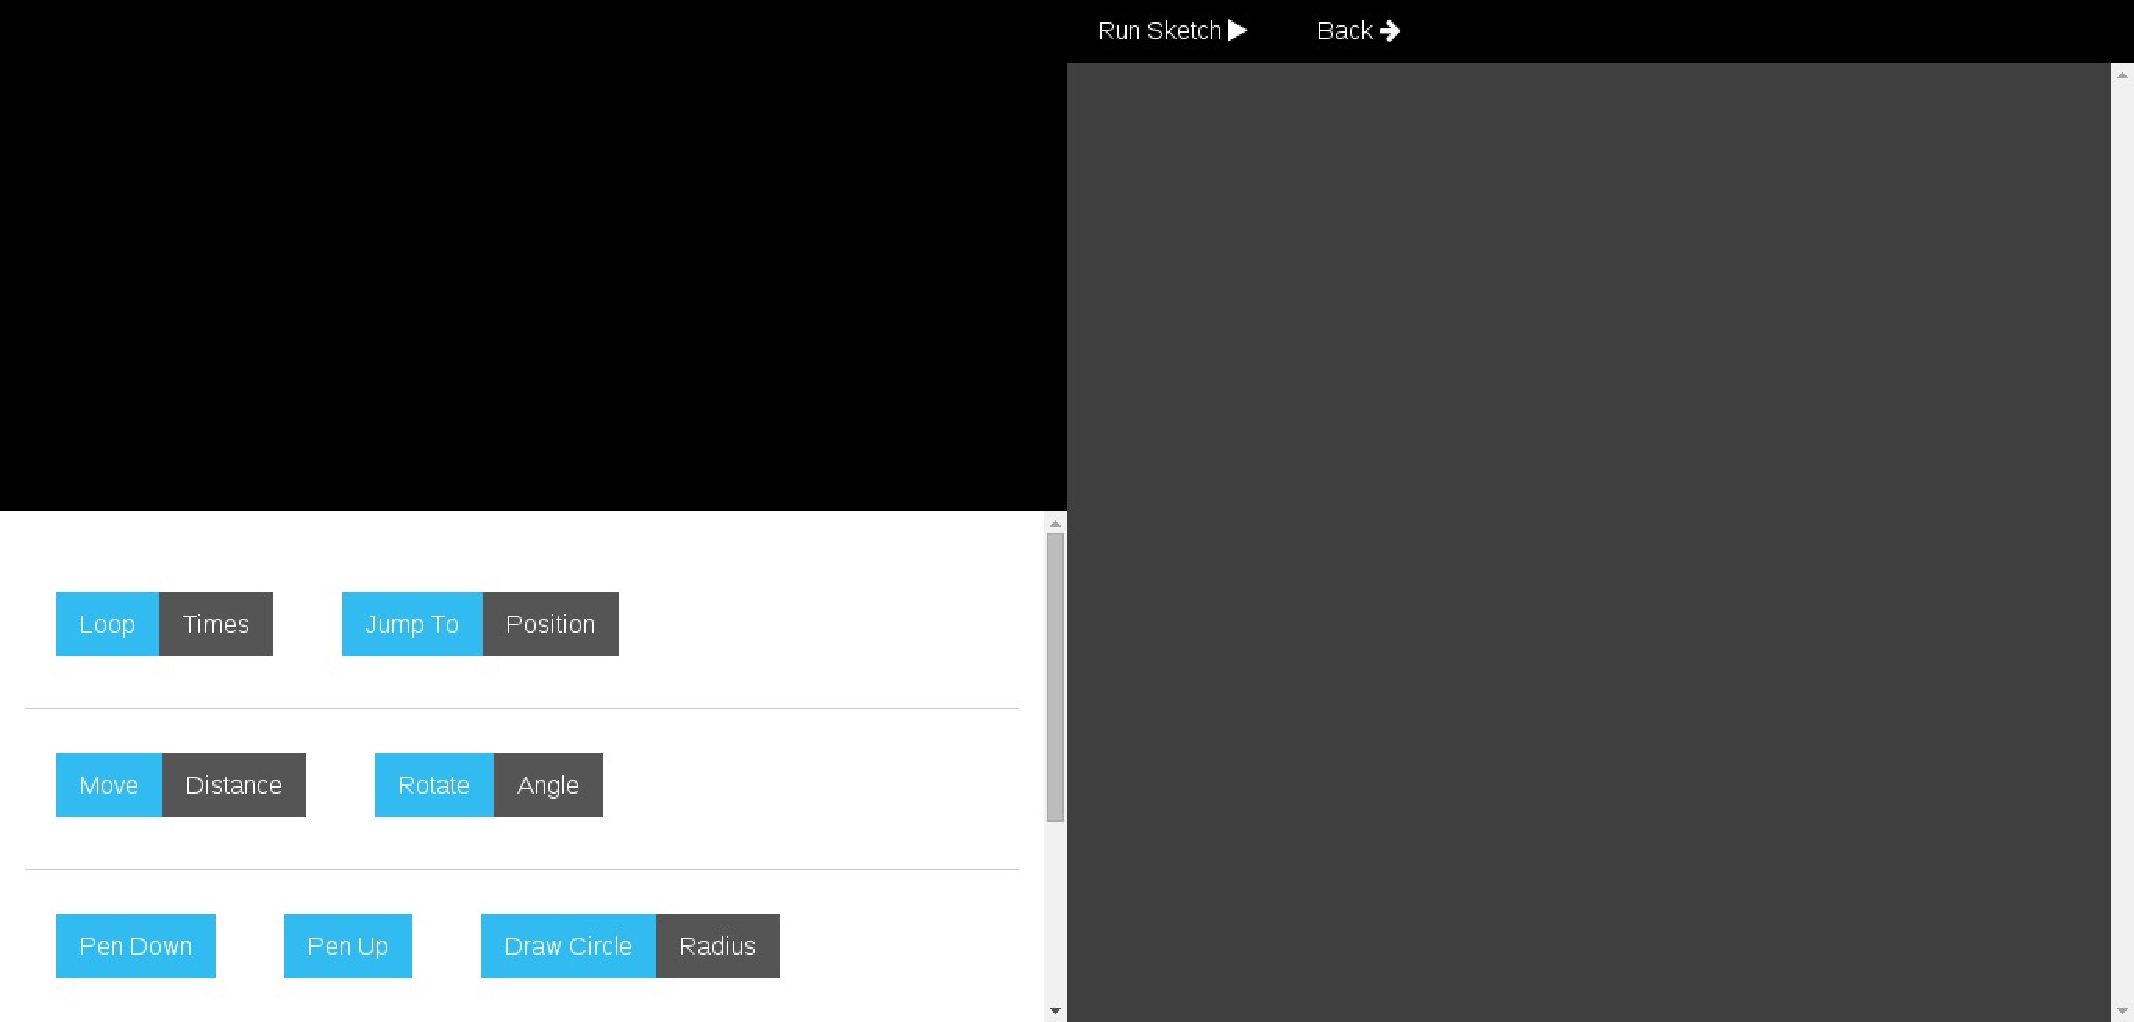
\includegraphics[width=\textwidth,keepaspectratio]{editor.pdf}
      \caption{Sketch Editor}
      \label{fig:axbgrid}
    \end{figure}
  \end{frame}

  \begin{frame}
    \frametitle{Frontend}
    \begin{figure}[h]
      \centering
      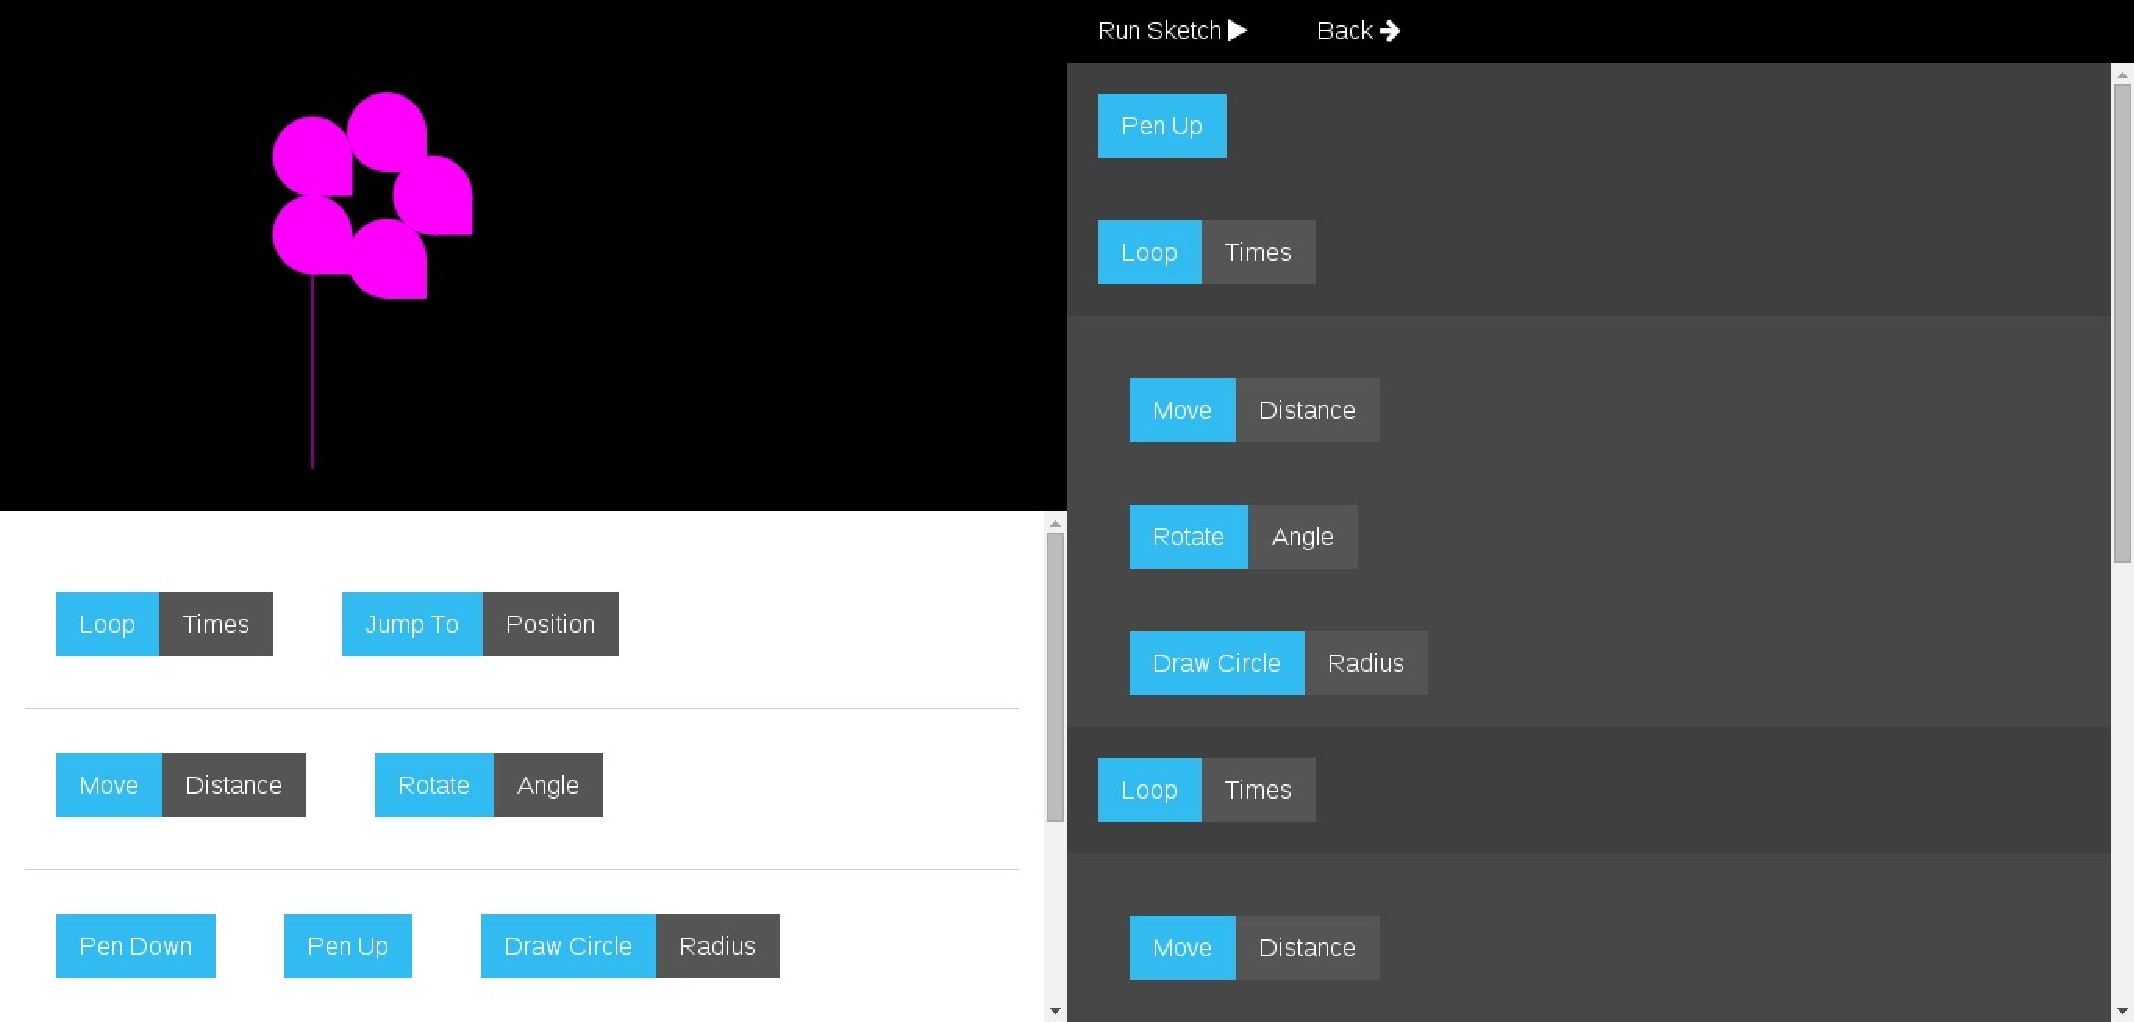
\includegraphics[width=\textwidth,keepaspectratio]{editor_with_contents.pdf}
      \caption{Sketch Editor with Contents}
      \label{fig:axbgrid}
    \end{figure}
  \end{frame}

  \begin{frame}
    \frametitle{System Architecture}
    \begin{itemize}
      \item Hosted on Heroku.
      \item Logical tier is NodeJS.
      \item Data tier is PostgreSQL.
      \item Preview images stored on Amazon S3
    \end{itemize}
  \end{frame}

  \section{Issues}
  \begin{frame}
    \frametitle{Scalability}
      \begin{itemize}
        \item Stateless protocol.
        \item Client side computation.
        \begin{itemize}
          \item Sketches are rendered client side
          \item Images are encoded on the client side.
        \end{itemize}
        \item Caching
        \begin{itemize}
    	     \item User sketches are stored locally, as well as the server side
        \end{itemize}
       \end{itemize}
  \end{frame}

  \begin{frame}
    \frametitle{Security}
    \begin{itemize}
      \item SQL text Input presented to PostgreSQL is parametrized to sanitize and avoid SQL injection.
      \item Escaping on the client side to avoid XSS.
    \end{itemize}
    We have identified the need to provide authentication of devices to prevent unauthorized access to  user data.
  \end{frame}

  \begin{frame}
    \frametitle{Potential Vulnerabilities}
    \begin{itemize}
      \item Issues with binary blob for preview images
      \item XSS issues with user created sketch names
      \item CORF attacks due to the nature of the NodeJS backend
    \end{itemize}
  \end{frame}

  \begin{frame}
    \frametitle{Reliability}
    \begin{itemize}
      \item Running on Heroku.
      \item Testing
      \item Strategies for dealing with DOS
        \begin{itemize}
          \item Rate limiting?
          \item Data constraints?
        \end{itemize}
    \end{itemize}
  \end{frame}

  \begin{frame}
    \frametitle{Privacy}
    \begin{itemize}
      \item Where we can, we have avoided coming into contact with private data
      \item Only store UUID which links back to device
      \item This UUID is masked behind a randomly chosen name and is never shown to any client
    \end{itemize}
  \end{frame}

  \begin{frame}
    \frametitle{Testing}
    \begin{itemize}
      \item CURL scripts for automated testing of routes
      \item Fuzzing to attempt to discover vulnerabilities
      \item Stress testing for reliability
    \end{itemize}
  \end{frame}

  \begin{frame}
    \frametitle{Still to do?}
    \begin{itemize}
      \item Integration between client and server side
      \item Potentially sharing of sketches on social media
    \end{itemize}
  \end{frame}

  \begin{frame}
    \frametitle{Responsibilities}
  \end{frame}
\end{document}
